\documentclass[]{book}
\usepackage{lmodern}
\usepackage{amssymb,amsmath}
\usepackage{ifxetex,ifluatex}
\usepackage{fixltx2e} % provides \textsubscript
\ifnum 0\ifxetex 1\fi\ifluatex 1\fi=0 % if pdftex
  \usepackage[T1]{fontenc}
  \usepackage[utf8]{inputenc}
\else % if luatex or xelatex
  \ifxetex
    \usepackage{mathspec}
  \else
    \usepackage{fontspec}
  \fi
  \defaultfontfeatures{Ligatures=TeX,Scale=MatchLowercase}
\fi
% use upquote if available, for straight quotes in verbatim environments
\IfFileExists{upquote.sty}{\usepackage{upquote}}{}
% use microtype if available
\IfFileExists{microtype.sty}{%
\usepackage{microtype}
\UseMicrotypeSet[protrusion]{basicmath} % disable protrusion for tt fonts
}{}
\usepackage[margin=1in]{geometry}
\usepackage{hyperref}
\hypersetup{unicode=true,
            pdftitle={Análisis multivariante de la comunidad},
            pdfauthor={Carlos Iván Espinosa},
            pdfborder={0 0 0},
            breaklinks=true}
\urlstyle{same}  % don't use monospace font for urls
\usepackage{natbib}
\bibliographystyle{apalike}
\usepackage{color}
\usepackage{fancyvrb}
\newcommand{\VerbBar}{|}
\newcommand{\VERB}{\Verb[commandchars=\\\{\}]}
\DefineVerbatimEnvironment{Highlighting}{Verbatim}{commandchars=\\\{\}}
% Add ',fontsize=\small' for more characters per line
\usepackage{framed}
\definecolor{shadecolor}{RGB}{248,248,248}
\newenvironment{Shaded}{\begin{snugshade}}{\end{snugshade}}
\newcommand{\KeywordTok}[1]{\textcolor[rgb]{0.13,0.29,0.53}{\textbf{{#1}}}}
\newcommand{\DataTypeTok}[1]{\textcolor[rgb]{0.13,0.29,0.53}{{#1}}}
\newcommand{\DecValTok}[1]{\textcolor[rgb]{0.00,0.00,0.81}{{#1}}}
\newcommand{\BaseNTok}[1]{\textcolor[rgb]{0.00,0.00,0.81}{{#1}}}
\newcommand{\FloatTok}[1]{\textcolor[rgb]{0.00,0.00,0.81}{{#1}}}
\newcommand{\ConstantTok}[1]{\textcolor[rgb]{0.00,0.00,0.00}{{#1}}}
\newcommand{\CharTok}[1]{\textcolor[rgb]{0.31,0.60,0.02}{{#1}}}
\newcommand{\SpecialCharTok}[1]{\textcolor[rgb]{0.00,0.00,0.00}{{#1}}}
\newcommand{\StringTok}[1]{\textcolor[rgb]{0.31,0.60,0.02}{{#1}}}
\newcommand{\VerbatimStringTok}[1]{\textcolor[rgb]{0.31,0.60,0.02}{{#1}}}
\newcommand{\SpecialStringTok}[1]{\textcolor[rgb]{0.31,0.60,0.02}{{#1}}}
\newcommand{\ImportTok}[1]{{#1}}
\newcommand{\CommentTok}[1]{\textcolor[rgb]{0.56,0.35,0.01}{\textit{{#1}}}}
\newcommand{\DocumentationTok}[1]{\textcolor[rgb]{0.56,0.35,0.01}{\textbf{\textit{{#1}}}}}
\newcommand{\AnnotationTok}[1]{\textcolor[rgb]{0.56,0.35,0.01}{\textbf{\textit{{#1}}}}}
\newcommand{\CommentVarTok}[1]{\textcolor[rgb]{0.56,0.35,0.01}{\textbf{\textit{{#1}}}}}
\newcommand{\OtherTok}[1]{\textcolor[rgb]{0.56,0.35,0.01}{{#1}}}
\newcommand{\FunctionTok}[1]{\textcolor[rgb]{0.00,0.00,0.00}{{#1}}}
\newcommand{\VariableTok}[1]{\textcolor[rgb]{0.00,0.00,0.00}{{#1}}}
\newcommand{\ControlFlowTok}[1]{\textcolor[rgb]{0.13,0.29,0.53}{\textbf{{#1}}}}
\newcommand{\OperatorTok}[1]{\textcolor[rgb]{0.81,0.36,0.00}{\textbf{{#1}}}}
\newcommand{\BuiltInTok}[1]{{#1}}
\newcommand{\ExtensionTok}[1]{{#1}}
\newcommand{\PreprocessorTok}[1]{\textcolor[rgb]{0.56,0.35,0.01}{\textit{{#1}}}}
\newcommand{\AttributeTok}[1]{\textcolor[rgb]{0.77,0.63,0.00}{{#1}}}
\newcommand{\RegionMarkerTok}[1]{{#1}}
\newcommand{\InformationTok}[1]{\textcolor[rgb]{0.56,0.35,0.01}{\textbf{\textit{{#1}}}}}
\newcommand{\WarningTok}[1]{\textcolor[rgb]{0.56,0.35,0.01}{\textbf{\textit{{#1}}}}}
\newcommand{\AlertTok}[1]{\textcolor[rgb]{0.94,0.16,0.16}{{#1}}}
\newcommand{\ErrorTok}[1]{\textcolor[rgb]{0.64,0.00,0.00}{\textbf{{#1}}}}
\newcommand{\NormalTok}[1]{{#1}}
\usepackage{longtable,booktabs}
\usepackage{graphicx,grffile}
\makeatletter
\def\maxwidth{\ifdim\Gin@nat@width>\linewidth\linewidth\else\Gin@nat@width\fi}
\def\maxheight{\ifdim\Gin@nat@height>\textheight\textheight\else\Gin@nat@height\fi}
\makeatother
% Scale images if necessary, so that they will not overflow the page
% margins by default, and it is still possible to overwrite the defaults
% using explicit options in \includegraphics[width, height, ...]{}
\setkeys{Gin}{width=\maxwidth,height=\maxheight,keepaspectratio}
\IfFileExists{parskip.sty}{%
\usepackage{parskip}
}{% else
\setlength{\parindent}{0pt}
\setlength{\parskip}{6pt plus 2pt minus 1pt}
}
\setlength{\emergencystretch}{3em}  % prevent overfull lines
\providecommand{\tightlist}{%
  \setlength{\itemsep}{0pt}\setlength{\parskip}{0pt}}
\setcounter{secnumdepth}{5}
% Redefines (sub)paragraphs to behave more like sections
\ifx\paragraph\undefined\else
\let\oldparagraph\paragraph
\renewcommand{\paragraph}[1]{\oldparagraph{#1}\mbox{}}
\fi
\ifx\subparagraph\undefined\else
\let\oldsubparagraph\subparagraph
\renewcommand{\subparagraph}[1]{\oldsubparagraph{#1}\mbox{}}
\fi

%%% Use protect on footnotes to avoid problems with footnotes in titles
\let\rmarkdownfootnote\footnote%
\def\footnote{\protect\rmarkdownfootnote}

%%% Change title format to be more compact
\usepackage{titling}

% Create subtitle command for use in maketitle
\newcommand{\subtitle}[1]{
  \posttitle{
    \begin{center}\large#1\end{center}
    }
}

\setlength{\droptitle}{-2em}
  \title{Análisis multivariante de la comunidad}
  \pretitle{\vspace{\droptitle}\centering\huge}
  \posttitle{\par}
  \author{Carlos Iván Espinosa}
  \preauthor{\centering\large\emph}
  \postauthor{\par}
  \predate{\centering\large\emph}
  \postdate{\par}
  \date{Octubre 2016}

\usepackage{booktabs}

\begin{document}
\maketitle

{
\setcounter{tocdepth}{1}
\tableofcontents
}
\chapter*{Prefacio}\label{prefacio}
\addcontentsline{toc}{chapter}{Prefacio}

\begin{center}\rule{0.5\linewidth}{\linethickness}\end{center}

qqqqqqqqqqqqqqqqqqqqqqqqqqqqqqqqqqqqqqqqqqqqqqqqqn el espacio y el
tiempo.

De esta forma la caracterización de una comunidad biológica se
constituye en un reto ya que implica poder rescatar los efectos que se
dan a varios niveles en la comunidad. El definir por ejemplo ¿Dónde
inicia y termina una comunidad? o ¿Cómo difieren las comunidades entre
localidades? o ¿Cómo la comunidad responde a las condiciones ambientales
o disturbios? representan algunas de las principales preguntas que
necesitamos responder. Una de las formas de responder estas preguntas
puede ser intentar cuantificar las similitudes entre localidades.

\chapter*{Objetivos}\label{objetivos}
\addcontentsline{toc}{chapter}{Objetivos}

\begin{center}\rule{0.5\linewidth}{\linethickness}\end{center}

\begin{itemize}
\item
  Comprender las bases teóricas para el cálculo de similitudes de la
  estructura de la comunidad entre localidades.
\item
  Utilizar herramientas de análisis para calcular índices de similitud y
  distancias entre comunidades.
\end{itemize}

\begin{figure}[htbp]
\centering
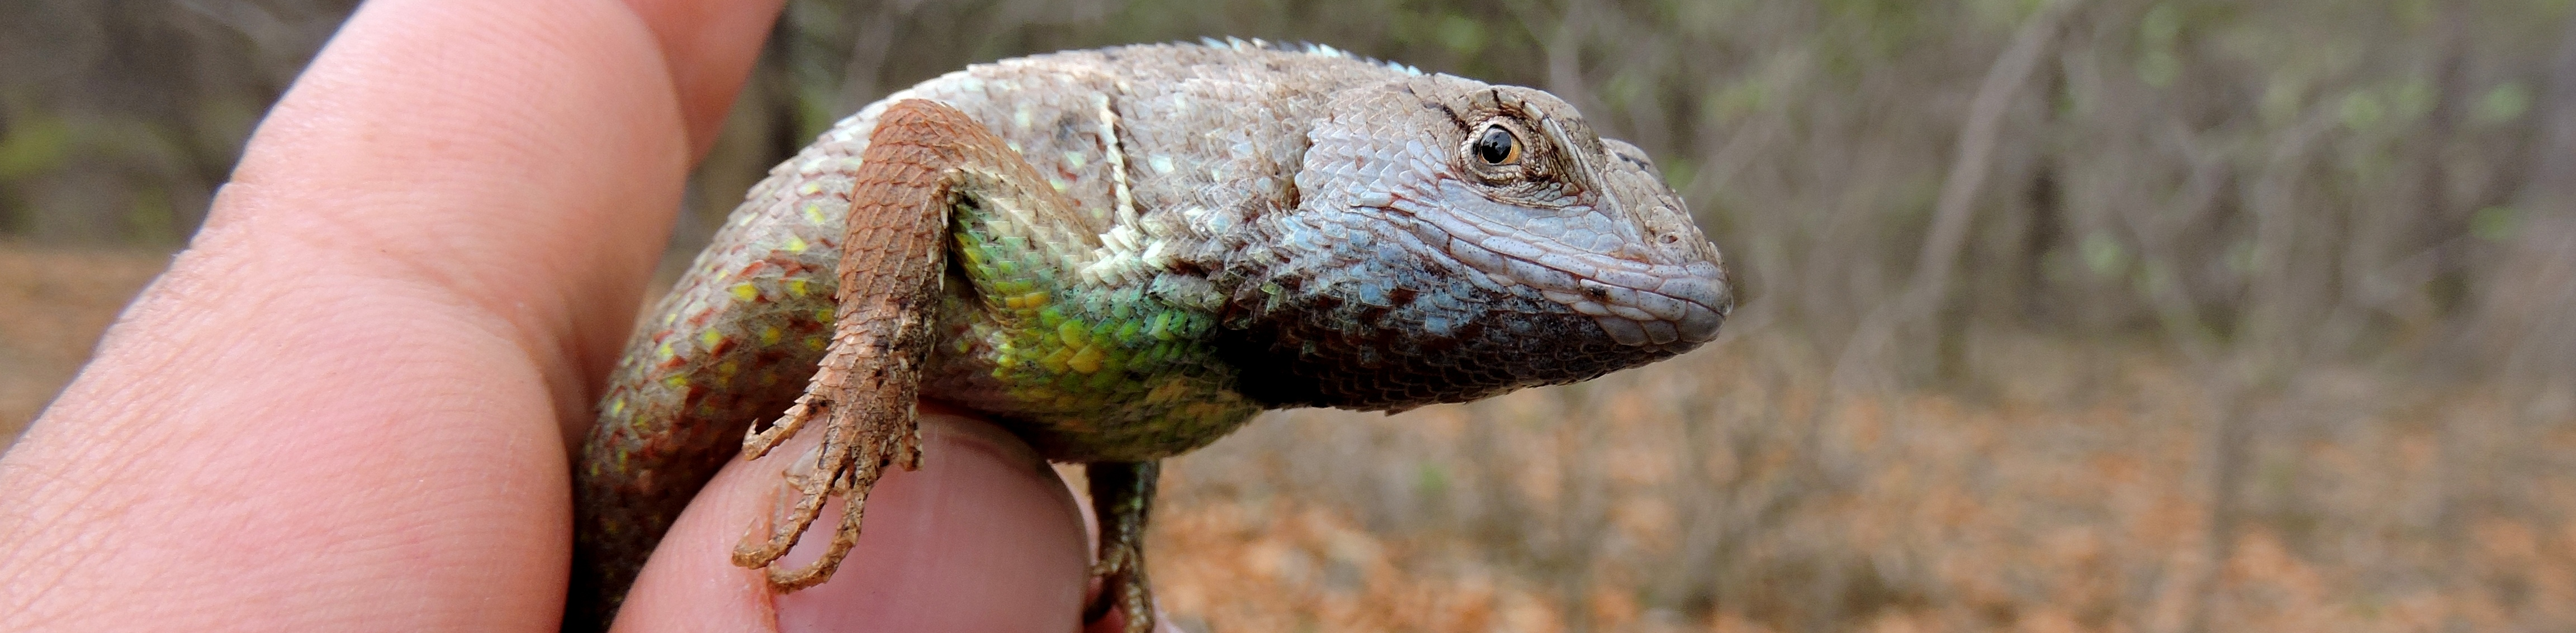
\includegraphics{lagar.jpg}
\caption{Stenocercus iridicens}
\end{figure}

\chapter{Medidas de similitud}\label{medidas-de-similitud}

\begin{center}\rule{0.5\linewidth}{\linethickness}\end{center}

La caracterización de una comunidad biológica presenta varios retos a
los ecólogos. ¿Dónde inicia y termina una comunidad? ¿Cómo difieren las
comunidades entre localidades? ¿Cómo la comunidad responde a las
condiciones ambientales o disturbios? ¿Cómo se mantiene la diversidad en
un área determinada? son algunas de las temáticas con mayor desarrollo
científico dentro de la ecología de comunidades. En el presente capítulo
se introduce a los estudiantes en los conceptos que los ecólogos
utilizan para comparar comunidades y se presenta una guía de algunos de
los análisis básicos de análisis de la estructura de las comunidades.

\section{Medidas de abundancia}\label{medidas-de-abundancia}

\begin{quote}
``La abundancia se refiere al número de individuos de una especie en una
determinada área''

--- (Smith and Smith 2010)
\end{quote}

Cuando hablamos de la composición de especies de una comunidad nos
referimos al conjunto de especies que habitan una determinada localidad.
Típicamente, esto incluye cierto grado de abundancia de cada especie,
pero puede también ser simplemente un listado de especies en esa
localidad, donde se registra la presencia o ausencia de cada especie.
Ahora, imaginemos que tenemos cuatro localidades (A, B, C, D) donde
recogemos los datos de densidad de dos especies; \emph{Tabebuia
billbergii} y \emph{Geofroea spinosa}, especies características de
bosques secos tropicales. Podemos introducir datos hipotéticos de
abundancia para cada especie en cada una de las localidades.

\begin{Shaded}
\begin{Highlighting}[]
\NormalTok{dens <-}\StringTok{ }\KeywordTok{data.frame}\NormalTok{(}\DataTypeTok{T.bil =} \KeywordTok{c}\NormalTok{(}\DecValTok{1}\NormalTok{, }\DecValTok{1}\NormalTok{, }\DecValTok{2}\NormalTok{, }\DecValTok{3}\NormalTok{), }\DataTypeTok{G.spi =} \KeywordTok{c}\NormalTok{(}\DecValTok{21}\NormalTok{, }\DecValTok{8}\NormalTok{, }\DecValTok{13}\NormalTok{, }\DecValTok{5}\NormalTok{)) }
\KeywordTok{row.names}\NormalTok{(dens) <-}\StringTok{ }\NormalTok{LETTERS[}\DecValTok{1}\NormalTok{:}\DecValTok{4}\NormalTok{]}
\NormalTok{dens}
\end{Highlighting}
\end{Shaded}

\begin{verbatim}
##   T.bil G.spi
## A     1    21
## B     1     8
## C     2    13
## D     3     5
\end{verbatim}

Generamos un gráfico para ver cuánto se parece cada sitio (Figura
\ref{fig:NMDS})

\begin{Shaded}
\begin{Highlighting}[]
\KeywordTok{par}\NormalTok{(}\DataTypeTok{mar=}\KeywordTok{c}\NormalTok{(}\DecValTok{4}\NormalTok{,}\DecValTok{4}\NormalTok{,}\DecValTok{1}\NormalTok{,}\DecValTok{1}\NormalTok{), }\DataTypeTok{mgp=}\KeywordTok{c}\NormalTok{(}\DecValTok{1}\NormalTok{,}\FloatTok{0.3}\NormalTok{,}\DecValTok{0}\NormalTok{), }\DataTypeTok{tcl=} \NormalTok{-}\FloatTok{0.2}\NormalTok{)}
\KeywordTok{plot}\NormalTok{(dens, }\DataTypeTok{type =} \StringTok{"n"}\NormalTok{, }\DataTypeTok{cex.axis=}\FloatTok{0.8}\NormalTok{) }
\KeywordTok{text}\NormalTok{(dens, }\KeywordTok{row.names}\NormalTok{(dens), }\DataTypeTok{col =}\StringTok{"blue"}\NormalTok{)}
\end{Highlighting}
\end{Shaded}

\begin{figure}[htbp]
\centering
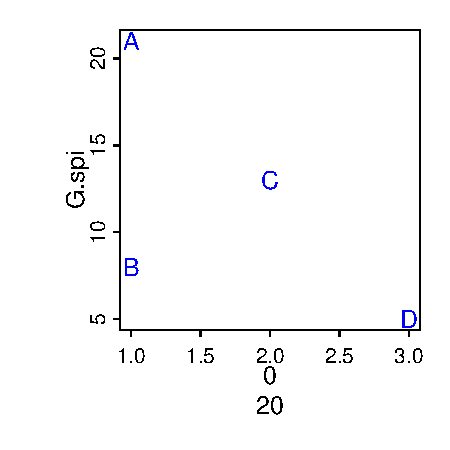
\includegraphics{bookdown-demo_files/figure-latex/NMDS-1.pdf}
\caption{\label{fig:NMDS}Distancias de cuatro localidades hipotéticas}
\end{figure}

En la Figura \ref{fig:NMDS} vemos que la composición de especies en el
sitio A es diferente de la composición del sitio D. Es decir, la
distancia entre el sitio A y D es mayor que entre los otros sitios. Lo
siguiente que nos deberíamos preguntar es; ¿qué tan distantes están los
dos sitios? Claramente, esto depende de la escala de medición (los
valores de los ejes), y sobre cómo medimos la distancia a través del
espacio multivariado \citep{Stevens2009}.

Estas diferencias entre sitios son dependientes de la abundancia de cada
especie. En el caso de \emph{G. spinosa} su eje varía entre 5 y 21,
mientras que para \emph{T. billbergii} varía entre 1 y 3. Una forma de
corregir esta distorsión es calcular la densidad relativa de cada
especie, de esta forma cada especie variará entre 0 y 1
\citep{Stevens2009}. Para ello dividimos la abundancia de cada especie
para la suma total de los individuos de las especies en esa muestra.

\begin{quote}
``La distancia se refiere a la diferencia en un espacio multidimensional
(dado por las especies) entre dos comunidades. Esta distancia puede ser
medida por múltiples vías''
\end{quote}

\begin{Shaded}
\begin{Highlighting}[]
\NormalTok{dens[}\DecValTok{1}\NormalTok{, ]/}\KeywordTok{sum}\NormalTok{(dens[}\DecValTok{1}\NormalTok{, ])}
\end{Highlighting}
\end{Shaded}

\begin{verbatim}
##        T.bil     G.spi
## A 0.04545455 0.9545455
\end{verbatim}

Este resultado nos muestra que el sitio A esta constituido en un 95\%
por \emph{G. spinosa}, mientras que \emph{T. billbergii} aporta
únicamente el 5\%. Cuando nos referimos a densidad relativa hablamos de
la densidad de una especie con referencia a algo, en el caso anterior
con referencia a otras especies en el mismo sitio, pero también
podríamos calcular en relación a otros sitios la misma especie.

\begin{Shaded}
\begin{Highlighting}[]
\NormalTok{dens[,}\DecValTok{1}\NormalTok{]/}\KeywordTok{sum}\NormalTok{(dens[,}\DecValTok{1}\NormalTok{])}
\end{Highlighting}
\end{Shaded}

\begin{verbatim}
## [1] 0.1428571 0.1428571 0.2857143 0.4285714
\end{verbatim}

Ahora podemos ver cómo \emph{T. billbergii} varía en su abundancia en
los cuatro sitios. El sitio A y B tienen el 14\% de individuos mientras
que el D tiene el 42\% de los individuos de esta especie.

Ya sea que nuestras medidas de abundancia son absoluta o relativa, nos
interesa conocer cuan diferente es la comunidad de una muestra (o sitio)
con relación a la otra. En el ejemplo ha sido fácil entender la
diferencia entre las dos comunidades debido a que teníamos únicamente
dos especies, pero con más de tres especies es complicado observar estas
diferencias gráficamente. Tal vez la forma más sencilla de describir la
diferencia entre los sitios es calcular las \emph{distancias} entre cada
par de sitios.

\section{Distancias entre sitios}\label{distancias-entre-sitios}

La \emph{distancia} entre dos muestras está dada por la diferencia entre
la abundancia y la composición de especies, como lo hemos visto esto
genera una distancia, en el caso del ejemplo la comunidad A esta más
alejada de la comunidad D que de las otras dos.

Existen muchas formas de poder calcular las distancias entre estos
puntos una de las más sencillas es la distancia \emph{Euclidiana}. La
distancia euclidiana entre dos sitios es simplemente la longitud del
vector que conecta los sitios y la podemos obtener como
\(\sqrt{x^2+y^2}\), donde \emph{``x''} y \emph{``y''} son las
coordenadas (x, y) de distancia entre un par de sitios.

En nuestro caso si queremos comparar B y C tenemos que la distancia en
el eje \emph{x} es la diferencia de la abundancia de \emph{T. bilbergii}
entre el sitio B y C.

\begin{Shaded}
\begin{Highlighting}[]
\NormalTok{x <-}\StringTok{ }\NormalTok{dens[}\DecValTok{2}\NormalTok{, }\DecValTok{1}\NormalTok{] -}\StringTok{ }\NormalTok{dens[}\DecValTok{3}\NormalTok{, }\DecValTok{1}\NormalTok{]}
\end{Highlighting}
\end{Shaded}

Mientras que la distancia en el eje \emph{y} es la diferencia en la
abundancia de \emph{G. spinosa} entre el sitio B y C.

\begin{Shaded}
\begin{Highlighting}[]
\NormalTok{y <-}\StringTok{ }\NormalTok{dens[}\DecValTok{2}\NormalTok{, }\DecValTok{2}\NormalTok{] -}\StringTok{ }\NormalTok{dens[}\DecValTok{3}\NormalTok{, }\DecValTok{2}\NormalTok{]}
\end{Highlighting}
\end{Shaded}

Ahora obtenemos las distancias entre los dos sitios

\begin{Shaded}
\begin{Highlighting}[]
\KeywordTok{sqrt}\NormalTok{(x^}\DecValTok{2} \NormalTok{+}\StringTok{ }\NormalTok{y^}\DecValTok{2}\NormalTok{)}
\end{Highlighting}
\end{Shaded}

\begin{verbatim}
## [1] 5.09902
\end{verbatim}

Pero como en \emph{R} todo es sencillo podemos utilizar la función
\emph{dist}

\begin{Shaded}
\begin{Highlighting}[]
\KeywordTok{dist}\NormalTok{(dens)}
\end{Highlighting}
\end{Shaded}

\begin{verbatim}
##           A         B         C
## B 13.000000                    
## C  8.062258  5.099020          
## D 16.124515  3.605551  8.062258
\end{verbatim}

Si bien este cálculo es sencillo con dos especies, si tenemos que
calcular la distancia para una comunidad con más de tres especies los
cálculos son tediosos y largos. Para calcular la distancia
\emph{Euclidiana} entre pares de sitios con \emph{R} especies utilizamos
la siguiente ecuación:

\begin{quote}
\[D_E = \sqrt{\sum_{i=l}^R (x_{ai} - x_{bi})^2}\] Distancia Euclidiana
\end{quote}

Existen otras formas de medir distancias entre dos localidades. En
ecología una de las distancias más utilizada es la distancia de
\emph{Bray-Curtis}, conocida también como \emph{Sorensen}. Esta
distancia es calculada como:

\begin{quote}
\[D_{BC} = \sum_{i=l}^R \frac{(x_{ai} - x_{bi})}{(x_{ai} + x_{bi})}\]
Distancia de Bray-Curtis
\end{quote}

La distancia \emph{Bray-Curtis} no es más que la diferencia total en la
abundancia de especies entre dos sitios, dividido para la abundancia
total en cada sitio. La distancia Bray-Curtis tiende a resultar más
intuitiva debido a que las especies comunes y raras tienen pesos
relativamente similares, mientras que la distancia euclidia depende en
mayor medida de las especies más abundantes. Esto sucede porque las
distancias euclidianas se basan en diferencias al cuadrado, mientras que
Bray-Curtis utiliza diferencias absolutas. El elevar un número al
cuadrado siempre amplifica la importancia de los valores más grandes. En
la figura \ref{fig:bray} se compara gráficos basados en distancias
euclidianas y Bray-Curtis de los mismos datos.

Como se había comentado es virtualmente imposible representar una
distancia en más de tres dimensiones (cada especie es una dimensión).
Una forma sencilla de mostrar distancias para tres o más especies es
crear un gráfico de dos dimensiones, intentando organizar todos los
sitios para que las distancias sean aproximadamente las correctas. Está
claro que esto es una aproximación nunca estas serán exactas. Una
técnica que intenta crear un arreglo aproximado es escalamiento
multidimensional no métrico (NMDS). Vamos a calcular las distancias para
nuestra comunidad, primero vamos a añadir dos especies más a nuestra
comunidad, \emph{Ceiba trichistandra} y \emph{Colicodendron scabridum}.

\begin{Shaded}
\begin{Highlighting}[]
\NormalTok{dens$C.tri<-}\StringTok{ }\KeywordTok{c}\NormalTok{(}\DecValTok{11}\NormalTok{, }\DecValTok{3}\NormalTok{, }\DecValTok{7}\NormalTok{, }\DecValTok{5}\NormalTok{)}
\NormalTok{dens$C.sca<-}\StringTok{ }\KeywordTok{c}\NormalTok{(}\DecValTok{16}\NormalTok{, }\DecValTok{0}\NormalTok{, }\DecValTok{9}\NormalTok{, }\DecValTok{4}\NormalTok{)}
\end{Highlighting}
\end{Shaded}

La función de escalamiento multidimensional no-métrico está en el
paquete \texttt{vegan}. Aquí mostramos las distancias euclidianas entre
sitios (Figura \ref{fig:bray}a) y las distancias de Bray-Curtis (Figura
\ref{fig:bray}b).

\begin{Shaded}
\begin{Highlighting}[]
\KeywordTok{library}\NormalTok{(vegan) }

\CommentTok{#Distancia Euclidiana}
\NormalTok{mdsE <-}\StringTok{ }\KeywordTok{metaMDS}\NormalTok{(dens, }\DataTypeTok{distance =} \StringTok{"euc"}\NormalTok{, }\DataTypeTok{autotransform =} \OtherTok{FALSE}\NormalTok{, }\DataTypeTok{trace =} \DecValTok{0}\NormalTok{) }
\CommentTok{#Distancia de Bray-Curtis}
\NormalTok{mdsB <-}\StringTok{ }\KeywordTok{metaMDS}\NormalTok{(dens, }\DataTypeTok{distance =} \StringTok{"bray"}\NormalTok{, }\DataTypeTok{autotransform =} \OtherTok{FALSE}\NormalTok{, }\DataTypeTok{trace =} \DecValTok{0}\NormalTok{) }
\end{Highlighting}
\end{Shaded}

\begin{Shaded}
\begin{Highlighting}[]
\KeywordTok{par}\NormalTok{(}\DataTypeTok{mfcol=}\KeywordTok{c}\NormalTok{(}\DecValTok{1}\NormalTok{,}\DecValTok{2}\NormalTok{), }\DataTypeTok{oma=}\KeywordTok{c}\NormalTok{(}\DecValTok{1}\NormalTok{,}\DecValTok{1}\NormalTok{,}\DecValTok{1}\NormalTok{,}\DecValTok{1}\NormalTok{), }\DataTypeTok{mar=}\KeywordTok{c}\NormalTok{(}\DecValTok{4}\NormalTok{,}\DecValTok{4}\NormalTok{,}\DecValTok{1}\NormalTok{,}\DecValTok{1}\NormalTok{),}
    \DataTypeTok{mgp=}\KeywordTok{c}\NormalTok{(}\DecValTok{1}\NormalTok{,}\FloatTok{0.3}\NormalTok{,}\DecValTok{0}\NormalTok{), }\DataTypeTok{tcl=} \NormalTok{-}\FloatTok{0.2}\NormalTok{)}

\KeywordTok{plot}\NormalTok{(mdsE, }\DataTypeTok{display =} \StringTok{"sites"}\NormalTok{, }
     \DataTypeTok{type =} \StringTok{"text"}\NormalTok{,}\DataTypeTok{main=}\StringTok{"a)Euclidiana"}\NormalTok{, }
     \DataTypeTok{cex.axis=} \FloatTok{0.7}\NormalTok{, }\DataTypeTok{cex.main=}\FloatTok{0.75}\NormalTok{, }\DataTypeTok{cex.lab=}\FloatTok{0.7}\NormalTok{)}

\KeywordTok{plot}\NormalTok{(mdsB, }\DataTypeTok{display =} \StringTok{"sites"}\NormalTok{, }\DataTypeTok{type =} \StringTok{"text"}\NormalTok{, }
     \DataTypeTok{main=}\StringTok{"b)Bray-Curtis"}\NormalTok{, }
     \DataTypeTok{cex.axis=} \FloatTok{0.7}\NormalTok{, }\DataTypeTok{cex.main=}\FloatTok{0.75}\NormalTok{, }\DataTypeTok{cex.lab=}\FloatTok{0.7}\NormalTok{)}
\end{Highlighting}
\end{Shaded}

\begin{figure}[htbp]
\centering
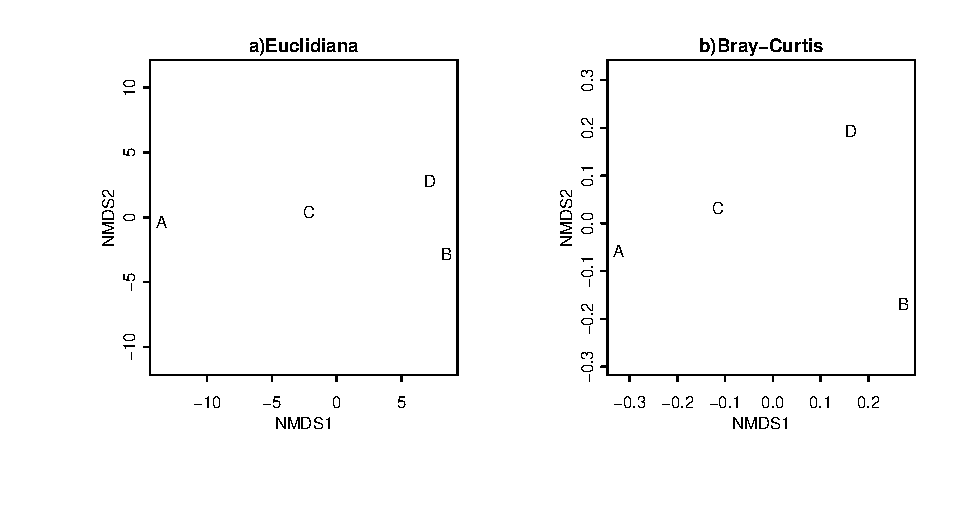
\includegraphics{bookdown-demo_files/figure-latex/bray-1.pdf}
\caption{\label{fig:bray}Arreglo de las parcelas en distancias
multidimensionales no métricas (NMDS). Estas dos figuras muestran los
mismos datos en bruto, pero las distancias euclidianas tienden a
enfatizar las diferencias debidas a las especies más abundantes,
mientras que Bray-Curtis no lo hace.}
\end{figure}

\section{Similitud}\label{similitud}

Ahora que sabemos cuan distantes son los diferentes sitios, muchas veces
nos podría interesar cuan similares son cada uno de los sitios a
continuación se describen dos medidas de similitud; \emph{Porcentaje de
Similitud} e \emph{Índice de Sorensen}.

El \emph{porcentaje de similitud} puede ser simplemente la suma de los
porcentajes mínimos de cada especie en la comunidad. Lo primero que
debemos hacer es convertir la abundancia de cada especie a su abundancia
relativa dentro de cada sitio. Para ello dividimos la abundancia de cada
especie por la suma de las abundancias en cada sitio.

\begin{Shaded}
\begin{Highlighting}[]
\NormalTok{dens.RA <-}\StringTok{ }\KeywordTok{t}\NormalTok{(}\KeywordTok{apply}\NormalTok{(dens, }\DecValTok{1}\NormalTok{, function(sp.abun) sp.abun/}\KeywordTok{sum}\NormalTok{(sp.abun)))}
\NormalTok{dens.RA}
\end{Highlighting}
\end{Shaded}

\begin{verbatim}
##        T.bil     G.spi     C.tri     C.sca
## A 0.02040816 0.4285714 0.2244898 0.3265306
## B 0.08333333 0.6666667 0.2500000 0.0000000
## C 0.06451613 0.4193548 0.2258065 0.2903226
## D 0.17647059 0.2941176 0.2941176 0.2352941
\end{verbatim}

El siguiente paso para comparar entre sitios, es encontrar el valor
mínimo para cada especie entre los sitios que debemos comparar. Vamos a
comparar los sitios A y B, para esto utilizamos la función
\texttt{aplly}, la cual nos permite encontrar el valor mínimo entre las
filas 1 y 2 (sitio A y B respectivamente). Para \emph{T. billbergi} en
el sitio A la abundancia relativa es 0.02 que es menor a la abundancia
en el sitio B que es de 0.08.

\begin{Shaded}
\begin{Highlighting}[]
\NormalTok{mins <-}\StringTok{ }\KeywordTok{apply}\NormalTok{(dens.RA[}\DecValTok{1}\NormalTok{:}\DecValTok{2}\NormalTok{, ], }\DecValTok{2}\NormalTok{, min)}
\NormalTok{mins}
\end{Highlighting}
\end{Shaded}

\begin{verbatim}
##      T.bil      G.spi      C.tri      C.sca 
## 0.02040816 0.42857143 0.22448980 0.00000000
\end{verbatim}

Finalmente para conocer el porcentaje de similitud entre los dos sitios
sumamos estos valores y multiplicamos por 100.

\begin{Shaded}
\begin{Highlighting}[]
\KeywordTok{sum}\NormalTok{(mins)*}\DecValTok{100}
\end{Highlighting}
\end{Shaded}

\begin{verbatim}
## [1] 67.34694
\end{verbatim}

Esto significa que la comunidad A y B tienen un porcentaje de similitud
del 67\%.

El índice de Sorensen es la segunda medida de similitud que vamos a
estudiar, este índice es medido como:

\begin{quote}
\[S_s= \frac{(2C)}{(A+B)}\] Índice de Sorensen
\end{quote}

Donde \emph{C} es el número de especies en común entre los dos sitios, y
\emph{A} y \emph{B} son el número de especies en cada sitio. Esto es
equivalente a dividir las especies compartidas por la riqueza media.

Para calcular el índice de Sorensen entre los sitios A y B necesitamos
definir el número de especies compartidas y luego la riqueza de cada uno
de los dos sitios.

Definimos si alguna de las especies en uno de los sitios la abundancia
no es igual a cero, eso nos dirá en qué casos se comparten especies.
Finalmente, sumamos todas las especies que su abundancia es mayor a
cero.

\begin{Shaded}
\begin{Highlighting}[]
\NormalTok{comp<-}\StringTok{ }\KeywordTok{apply}\NormalTok{(dens[}\DecValTok{1}\NormalTok{:}\DecValTok{2}\NormalTok{, ], }\DecValTok{2}\NormalTok{, function(abuns) }\KeywordTok{all}\NormalTok{(abuns !=}\StringTok{ }\DecValTok{0}\NormalTok{))}
\NormalTok{comp}
\end{Highlighting}
\end{Shaded}

\begin{verbatim}
## T.bil G.spi C.tri C.sca 
##  TRUE  TRUE  TRUE FALSE
\end{verbatim}

\begin{Shaded}
\begin{Highlighting}[]
\NormalTok{Rs <-}\StringTok{ }\KeywordTok{apply}\NormalTok{(dens[}\DecValTok{1}\NormalTok{:}\DecValTok{2}\NormalTok{, ], }\DecValTok{1}\NormalTok{, function(x) }\KeywordTok{sum}\NormalTok{(x >}\StringTok{ }\DecValTok{0}\NormalTok{))}
\NormalTok{Rs}
\end{Highlighting}
\end{Shaded}

\begin{verbatim}
## A B 
## 4 3
\end{verbatim}

Como vemos, la abundancia de \emph{C. scabridum} en uno de los dos
sitios es igual a Cero, lo confirmamos al tener la riqueza por sitio. El
sitio B tenemos únicamente 3 especies.

Ahora aplicamos la formula, dividimos las especies compartidas
(\emph{comp}) para la riqueza total de los dos sitios y lo multiplicamos
por 2.

\begin{Shaded}
\begin{Highlighting}[]
\NormalTok{(}\DecValTok{2}\NormalTok{*}\KeywordTok{sum}\NormalTok{(comp))/}\KeywordTok{sum}\NormalTok{(Rs)}
\end{Highlighting}
\end{Shaded}

\begin{verbatim}
## [1] 0.8571429
\end{verbatim}

Según el índice de Sorensen estos dos sitios son parecidos en un 86\%.
Los datos de los dos índices utilizados difieren entre sí, el porcentaje
de similitud utiliza no solamente la presencia ausencia sino también la
abundancia lo que podría estar reduciendo la similitud entre sitios.

\begin{center}\rule{0.5\linewidth}{\linethickness}\end{center}

\section{Ejercicio: Análisis de
similitud}\label{ejercicio-analisis-de-similitud}

\begin{center}\rule{0.5\linewidth}{\linethickness}\end{center}

Una de las preguntas básicas de un ecólogo es saber ¿Cómo de diferentes
son dos comunidades?, en el presente ejercicio nos interesa entender
comprender la similitud y distancias entre estas cinco comunidades
hipotéticas (tabla \ref{tab:ejer1} )

\begin{table}

\caption{\label{tab:ejer1}Comunidades hipotéticas}
\centering
\begin{tabular}[t]{lrrrrrrrr}
\toprule
  & sp1 & sp2 & sp3 & sp4 & sp5 & sp6 & sp7 & sp8\\
\midrule
A & 26 & 17 & 16 & 1995 & 159 & 0 & 362 & 0\\
B & 0 & 35 & 14 & 236 & 54 & 0 & 496 & 57\\
C & 24 & 0 & 26 & 17 & 88 & 18 & 907 & 20\\
D & 35 & 18 & 24 & 2033 & 175 & 15 & 376 & 16\\
E & 105 & 129 & 40 & 18 & 191 & 53 & 964 & 134\\
\bottomrule
\end{tabular}
\end{table}

Con los datos anteriores:

\begin{enumerate}
\def\labelenumi{\alph{enumi}.}
\item
  Convierta los datos en abundancia relativa por sitio (la suma en cada
  sitio debe ser igual a 1). Dibuje dos gráficas para representar; i) la
  abundancia total y ii) abundancia relativa de cada localidad. ¿Qué
  diferencias puede ver en la gráfica i y en la ii?
\item
  Calcule la distancia Euclideana y de Bray Curtis para cada sitio con
  las dos medidas de abundancia y grafíquelas utilizando el NMDS. ¿Cómo
  cambia entre distancias y abundancias? Explique las diferencias.
\item
  Evalúe la similitud (Sorensen) y el porcentaje de similitud entre
  pares de sitios. ¿Cuáles son los sitios más similares? ¿Cuál es la
  razón de las diferencias entre los índices utilizados?
\end{enumerate}

\bibliography{packages.bib}


\end{document}
